\section{Design}
\label{sec:design}

These processes of creating a core system, functionality flow, application architecture, and User Interface and Interaction; are definitely into \textit{design} process, sketching and mocking up.
Wireframing could be skipped since the design sketch is very simple, or really close resemble between the plan and expected result.

% --------------------------------------------------
\subsection{Contextual System}

To comply with the various shapes of knowledge context, there should be a feature system that can handle them.
It can be done with a major role of feature system that Satellid use called ``Contextual''.
The main system is by shortening the steps that needed to do a knowledge management that have context, naturally with making it more effective and accessible.

\begin{figure}[htb]
    \centering
    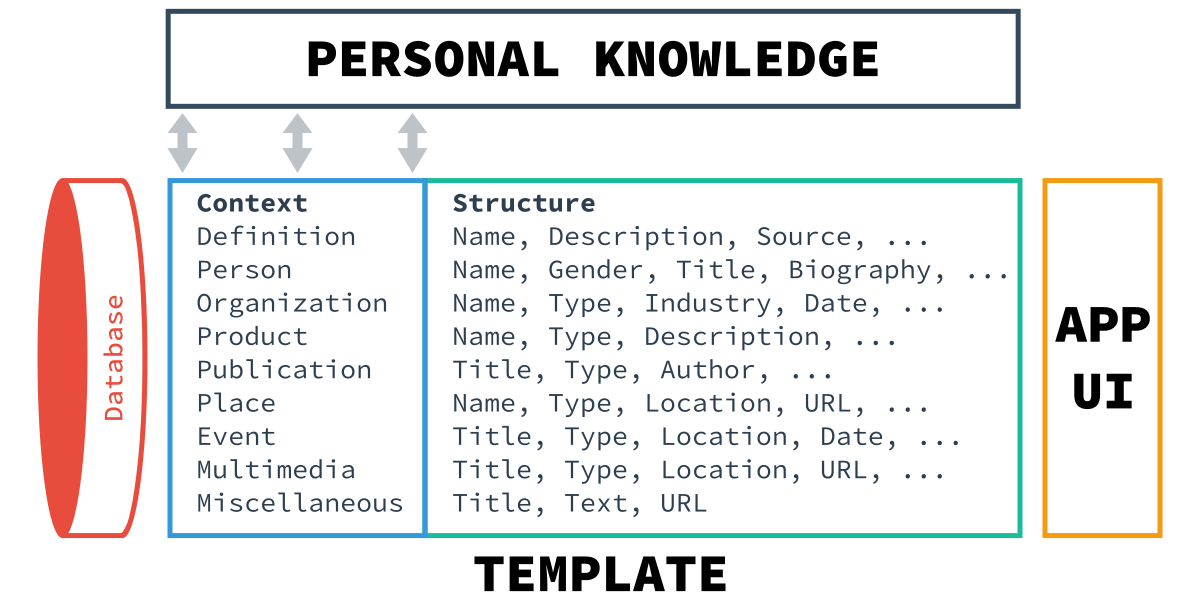
\includegraphics[width=\textwidth]{\dir/include/satellid-contextual.png}
    \caption{Satellid's Contextual system visual representation}
    \label{fig:satellid-contextual}
\end{figure}

Contextual, illustrated as in \autoref{fig:satellid-contextual}, utilize inputted knowledge and template that are used together to form the context and structure.
With this, user will eventually always structure their data, and even create more or modify available data field.
In addition to this, categorization and tagging could also be included and built.
The difference of context with category or tag is how it handles specificity.
Context is a very general descriptor so it can be fully understand and assess the content easily, rather than category or tag that is more widely and freely determined or should be specific.
Even though, a contexted knowledge could have category or tag.
For example, \textit{The Merriam-Webster Dictionary} may be categorized as a ``dictionary'', ``book'', ``reference'', ``glossary'', ``thesaurus'' and tagged as ``word'', ``language'', ``english'', ``''; but its context basically just a ``publication''.
So it can be in the same context like a \textit{O'Reilly Media's JavaScript, The Definitive Guide book} or even a \textit{Marvel's Iron Man comic}.
Contextual provide some of the most common type of knowledge with its key attributes.
The basic properties of metadata are including ID, Context, Date \& Time (Created \& Updated); while others are the Content or Detail.
As already defined, the lists below are the sorted version of prospected key attributes related to single context that needed and can be used.
Each of them can have category or label if appropriate, even additional custom text.
Also sometimes blank field is allowed like if there is unknown location and \ac{URL}, while in other condition multiple entries could occur.

\begin{easylist}
& Definition
  && Name, Description, Source, Author, URL
& Person
  && Name (Full, First, Last, Nick, Alias), Gender, Birth Date or Age, Title (Job), Biography, Location (Address, City, Country, \& Coordinates), Phone, Email, Website, URL
& Organization
  && Name, Type (School, University, Institution, Company, Group, Community, Band, etc), Industry, Date (Founded), Location (Address \& Coordinates), Product (their Services or Goods), URL
& Product
  && Name, Type (Service, Hardware, Software, Food, Clothing, etc), Tagline, Description, Brand Detail, URL
& Publication
  && Title, Type (Article, Book, Paper, Dictionary, Novel, Tutorial, Comic, Website, Blog, etc), Author, Description, URL
& Place
  && Name, Type (Station, Library, Park, Shop, Restaurant, Mall, Hotel, City, Country, etc), Location (Address \& Coordinates), URL
& Event
  && Title, Type (Meetup, Seminar, Workshop, Conference, Festival, etc), Location (Address), Date, Presenter, Sponsor, URL
& Multimedia
  && Title, Type (Photo, Image, Video, Film, etc), Location, Date and Time (Published), Duration, Creator, URL
& Miscellaneous
  && Title, Text, URL
\end{easylist}

Other contexts that still classified as miscellaneous or mixed are like Reminder, Story, Rules, Code, Requisites, Manifesto, random notes, etc.
Simply put, miscellaneous is the knowledge that have not been built its general context or other things that have not prespecified yet.

% --------------------------------------------------
\subsection{Functionality Flow}

Since the primary reason to build the implementation of Satellid is to enable daily knowledge management for personal, the main focus to enable that person who frequently get knowledge or wanted to store their knowledge in a simple manner.
The primary functionality is to do \ac{BREAD}, also without having to bother the entries arrangement and everything is managed in a predefined context.
The application could be just deployable via a local network (easily also in their own computer) or accessed from the Web via Internet.
In a very simple way of interaction, it should be very intuitive.
To keep the process faster and shorter, all of the functional process can be done in one single interface layout of the application.
It all could happen with a simplified unified interface.
So there is no need to switch back and forth to different views of browse, search, read, edit, add, and delete.

\noindent There are some terminologies or parts of the interaction used in this flow:
\vspace{-10pt}

\begin{description}
\item [User]: The primary person who use Satellid
\item [System]: The Satellid application
\item [Database]: The database that used by Satellid
\item [Knowledge]: The knowledge inside database that accessed and managed with Satellid
\item [Template]: The template to wrap the data schema
\item [Search bar]: The input that User can use to search for knowledge
\item [Buttons]: The input or modifier that User can use to add, edit, and delete a knowledge
\item [Knowledge Card]: The entity of a single knowledge framed with context, its object content
\item [Knowledge Collection]: The output that User can view the list of knowledge cards
\end{description}

\noindent The System will do the following flow:

\begin{enumerate}
\item System can be accessed and used by the User
\item System can run the desired interaction functionality by the User
\item System constantly monitor modification of Knowledge in the Database
\end{enumerate}

\noindent The User interactions are defined by these flow:

\begin{easylist}[enumerate]
& User can turn on and turn off the System.
& User can access and use the System.
& User can interact with the System to:
  && Browse the stored Knowledge.
  && Search a stored Knowledge.
  && Read a stored Knowledge.
  && Add a new Knowledge.
  && Edit a stored Knowledge.
  && Delete a stored Knowledge.
& When User enter a text into the search bar:
  && Search a Knowledge based on typed text string.
  && System search for matching text, automatically without having to press for a button.
  && If matched Text is found, System show the search result.
  && User get the found Knowledge.
& When User click/tap the add button beside the search bar:
  && Add a new knowledge based on its context.
  && User complete the new Knowldge.
  && If new Knowledge is successfully inputted, System store the new Knowledge into the System.
& When User click/tap the edit button beside the knowledge card:
  && Edit an existing knowledge.
  && User edit the Knowldge.
  && If the Knowledge is successfully edited, System store the edited Knowledge into the System.
& When User click/tap the delete button beside the knowledge card:
  && Delete an existing knowledge.
  && If the Knowledge is confirmed to be deleted, System delete the Knowledge from the System.
\end{easylist}

% --------------------------------------------------
\subsection{Application Architecture}

As previously known, the application architecture is heavily based on Meteor platform.
It also covers its stack such as the JavaScript platform (Node.js), NoSQL database (MongoDB), reactive protocol (DDP).
All of them run in a regular web application environment, which there are client-side and server-side connected via a network that can be Internet or local network.
Based on simple web application architecture, the application is architected as in \autoref{fig:satellid-app-arch}.

\begin{figure}[htbp]
    \centering
    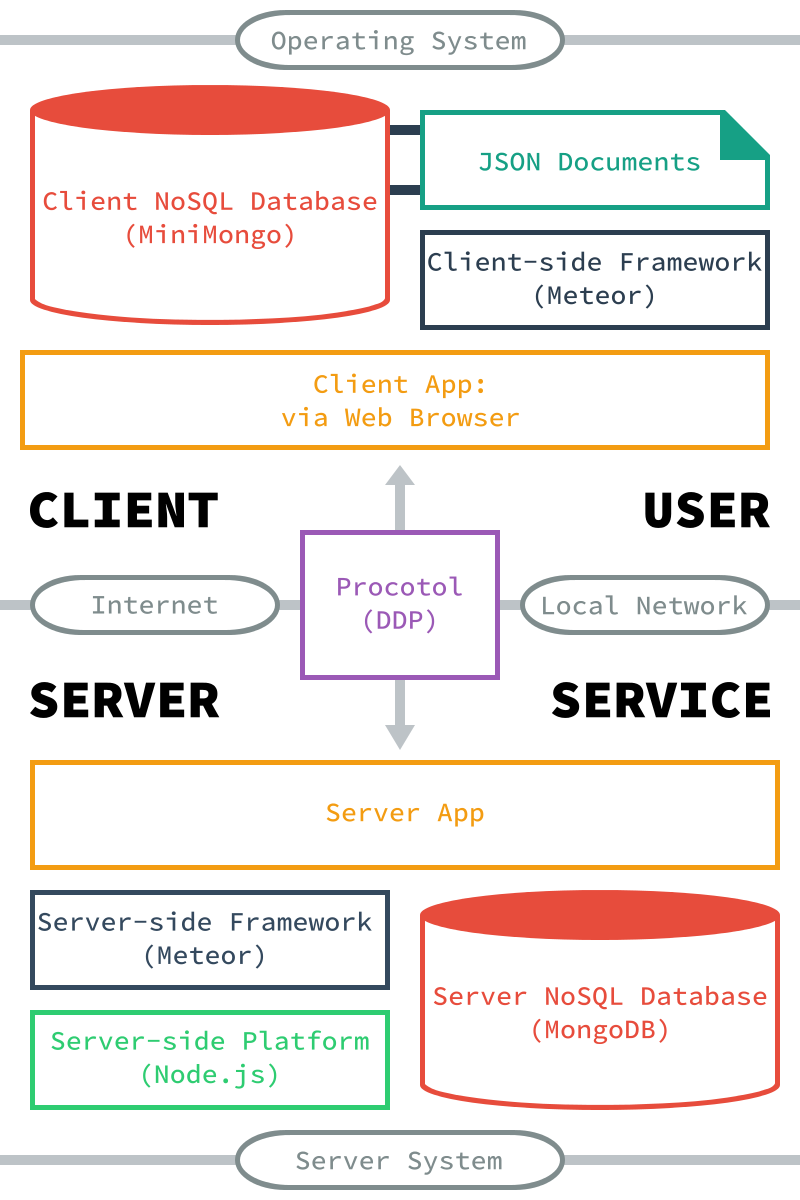
\includegraphics[width=8cm]{\dir/include/satellid-app-arch.png}
    \caption[Satellid Application Architecture]{The architecture of Satellid application}
    \label{fig:satellid-app-arch}
\end{figure}

The application started from the server system, running it including Node.js platform, Meteor platform, and server NoSQL database.
Those are served and accessed via the server-side app, naturally on top of a web server.
The application accessed by user from the client side, running it including Meteor app and client NoSQL database with \ac{JSON} documents that retrieved.
Those are accessible and enabled via client-side app, via the web browser.
Between the two, the protocol called \ac{DDP} maintain and manage the data transportation from server and client and from client to server.

% --------------------------------------------------
\subsection{User Interface and Interaction}

Here are the complete user interface and interaction on the web app version of Satellid.
The application main interface planning or \ac{UI} mockup design is laid out very simple with \ac{SPA} model/design, just like in \autoref{fig:satellid-app-ui}, including some mockups or example.
This \ac{UI} figures what the user see in the web app dimension.
And then, added with essentially the \ac{HCI} design or can be also a \ac{UIX} design.
The application main interaction or \ac{UIX} of each functionality flow of user interactions can be defined just like in \autoref{fig:satellid-app-ix}.
Note that these designs are intended mainly for the initial purpose of documentation only.
Since there is an agile works that perform in the development process, the design or documentation may change frequently and continuously for each iteration or modification, resulting a slightly different appearance within the actual implementation.

As seen in \autoref{fig:satellid-app-ui}, the \ac{UI} mockup design is really straightforward.
There is a logo on top of the interface.
The search bar is below the logo, then the add button is beside it.
The form box is the field to add knowledge.
All the knowledge collection that visualized in cards are beneath them.
Each knowledge card has a content, the knowledge

As seen in \autoref{fig:satellid-app-ix}, The \ac{UIX} design however is a bit more complex as it's explaining on how the application will be used.
Also it presents the design like a barebone structure with the process of the \ac{UI}.
In an unordered fashion, there are some interaction process that will be done like in the design.
Each components are annotated with actionable interaction and some detailed description or behavior.
Based on functionality flow, below are the available actions and explanation for User:

\begin{easylist}[enumerate]
& Turn on and turn off the System via terminal/\ac{CLI}.
& Access and use the System via Web browser.
& Type and search in the search bar that could automatically show the search result.
& Browse the existing knowledge or search result in the collection of cards.
& Add a knowledge that will show the form box to fill.
  && Choose a predefined context.
  && Fill each field with value that could be text, number, date-time, etc.
  && Save to store the knowledge.
  && Cancel to close the form box.
& Edit a knowledge with edit mode of form box.
  && Currently the context should and could not be changed, so there will be no collision between old and new content structure.
  && Each field except the header identity (name or title) is optional to fill.
& Delete a knowledge.
\end{easylist}

\begin{figure}[htb]
  \centering
  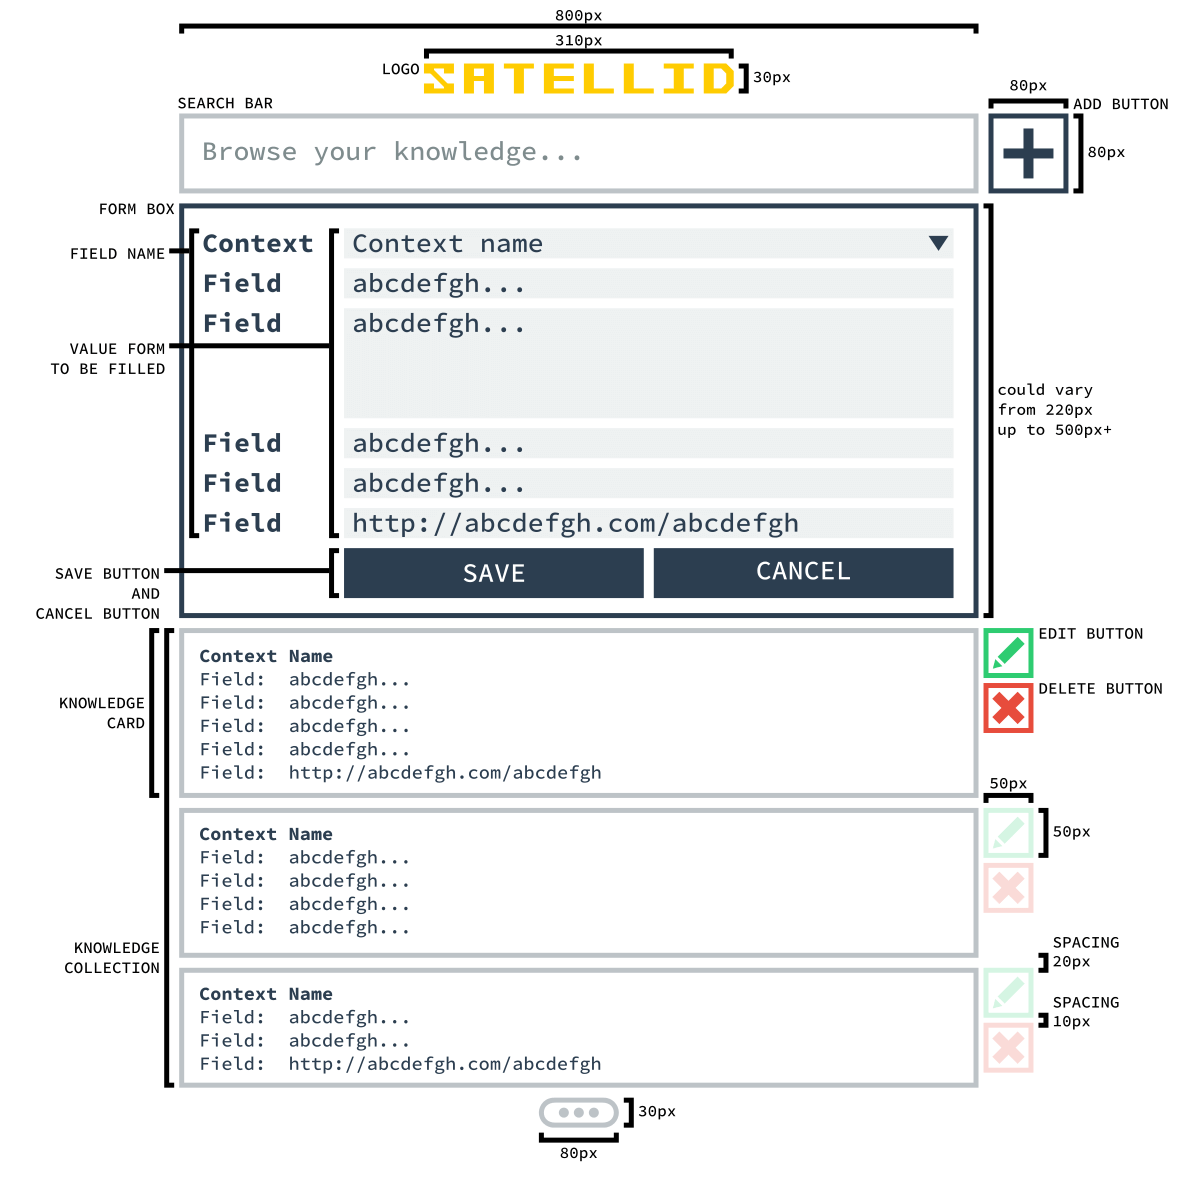
\includegraphics[width=\textwidth]{\dir/include/satellid-app-ui.png}
  \caption{Initial user interface mockup design of Satellid app}
  \label{fig:satellid-app-ui}
\end{figure}

\begin{figure}[htb]
  \centering
  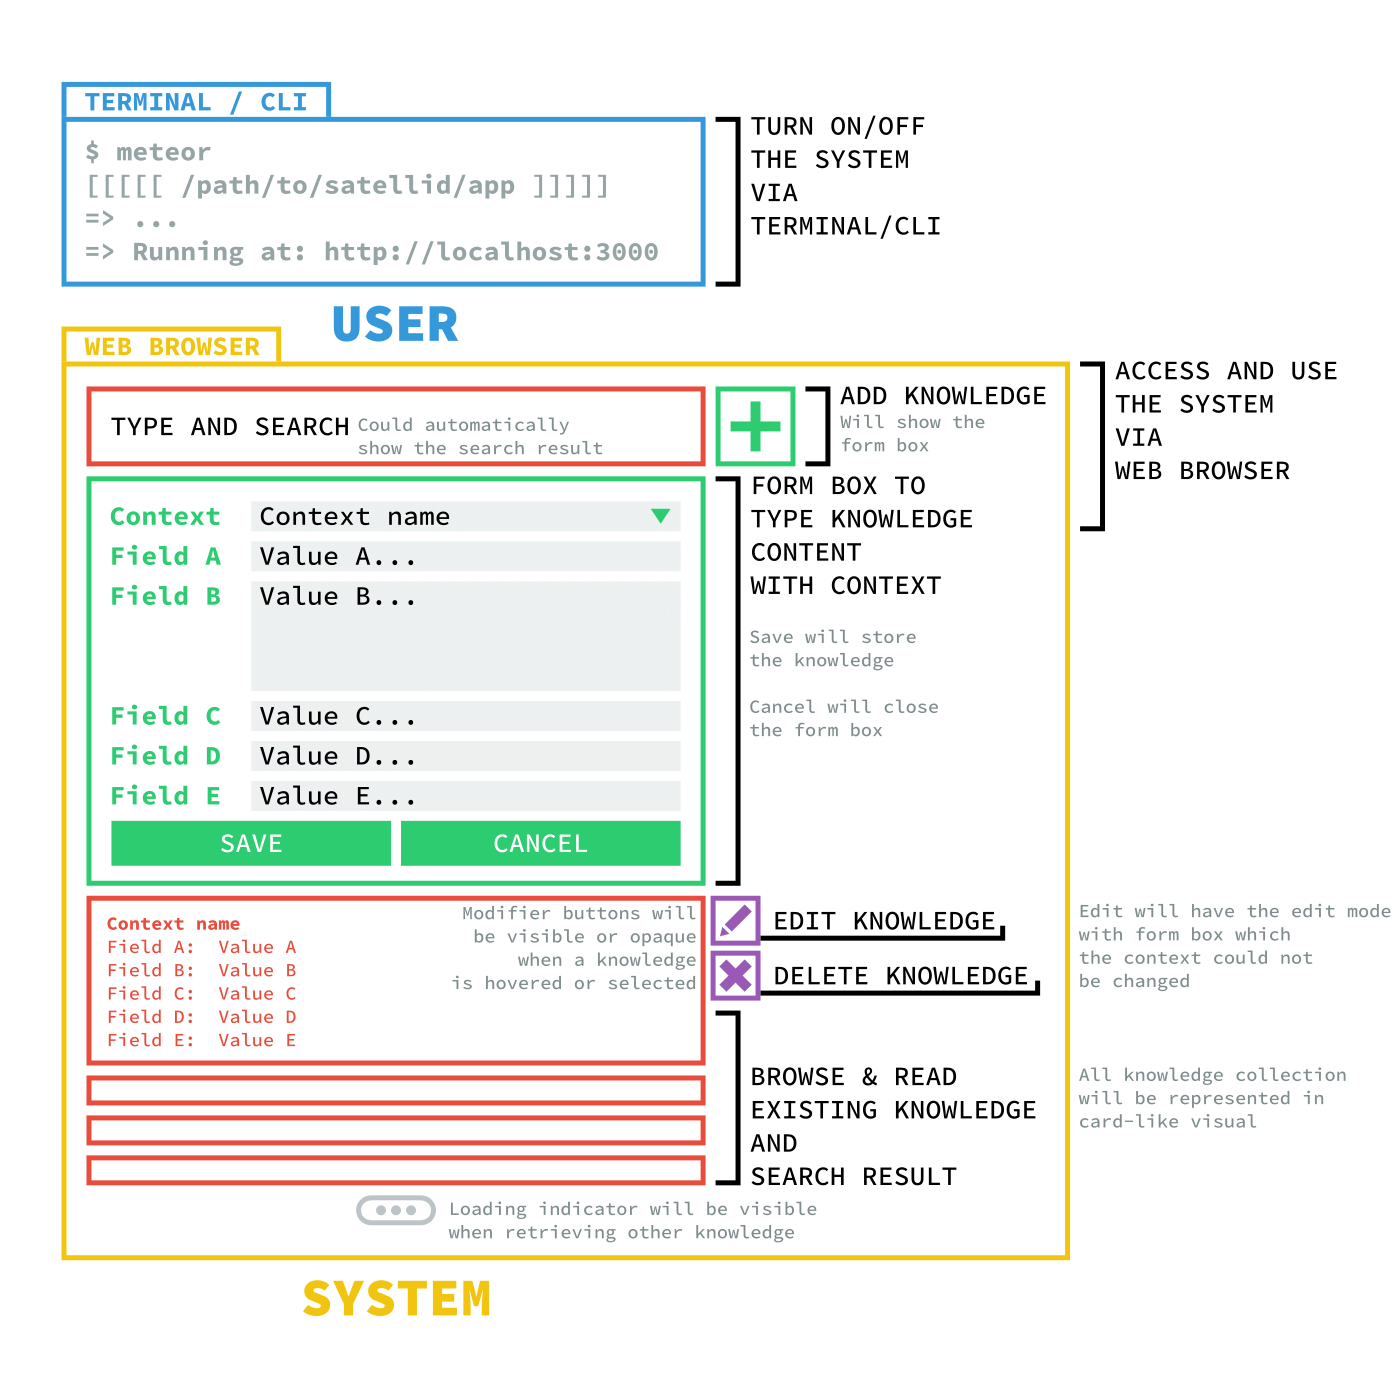
\includegraphics[width=15cm]{\dir/include/satellid-app-uix.png}
  \caption{Initial user interaction design of Satellid app}
  \label{fig:satellid-app-uix}
\end{figure}
